\Chapter{Tesztelés és Eredmények}

A program funkciói a fejlesztés során folyamatosan tesztelésre kerültek, alapvetően manuálisan. Az algoritmus, illetve a szemantikus verziózás tesztelése végül a statisztikai vizsgálat során automatikusan is megtörtént, bár nem ez volt annak a résznek a célja. Ennek következtében derült ki az algoritmusnál is tárgyalt hiba, miszerint nem számított bizonyos átlagtól eltérő esetekre, amely a ciklus végtelen futását eredményezte.\\

Ebben a szekcióban a program felhasználása, illetve a használatával szerzett eredmények elemzése kerül ismertetésre.

\Section{Használat}

\begin{figure}[!h]
	\centering
	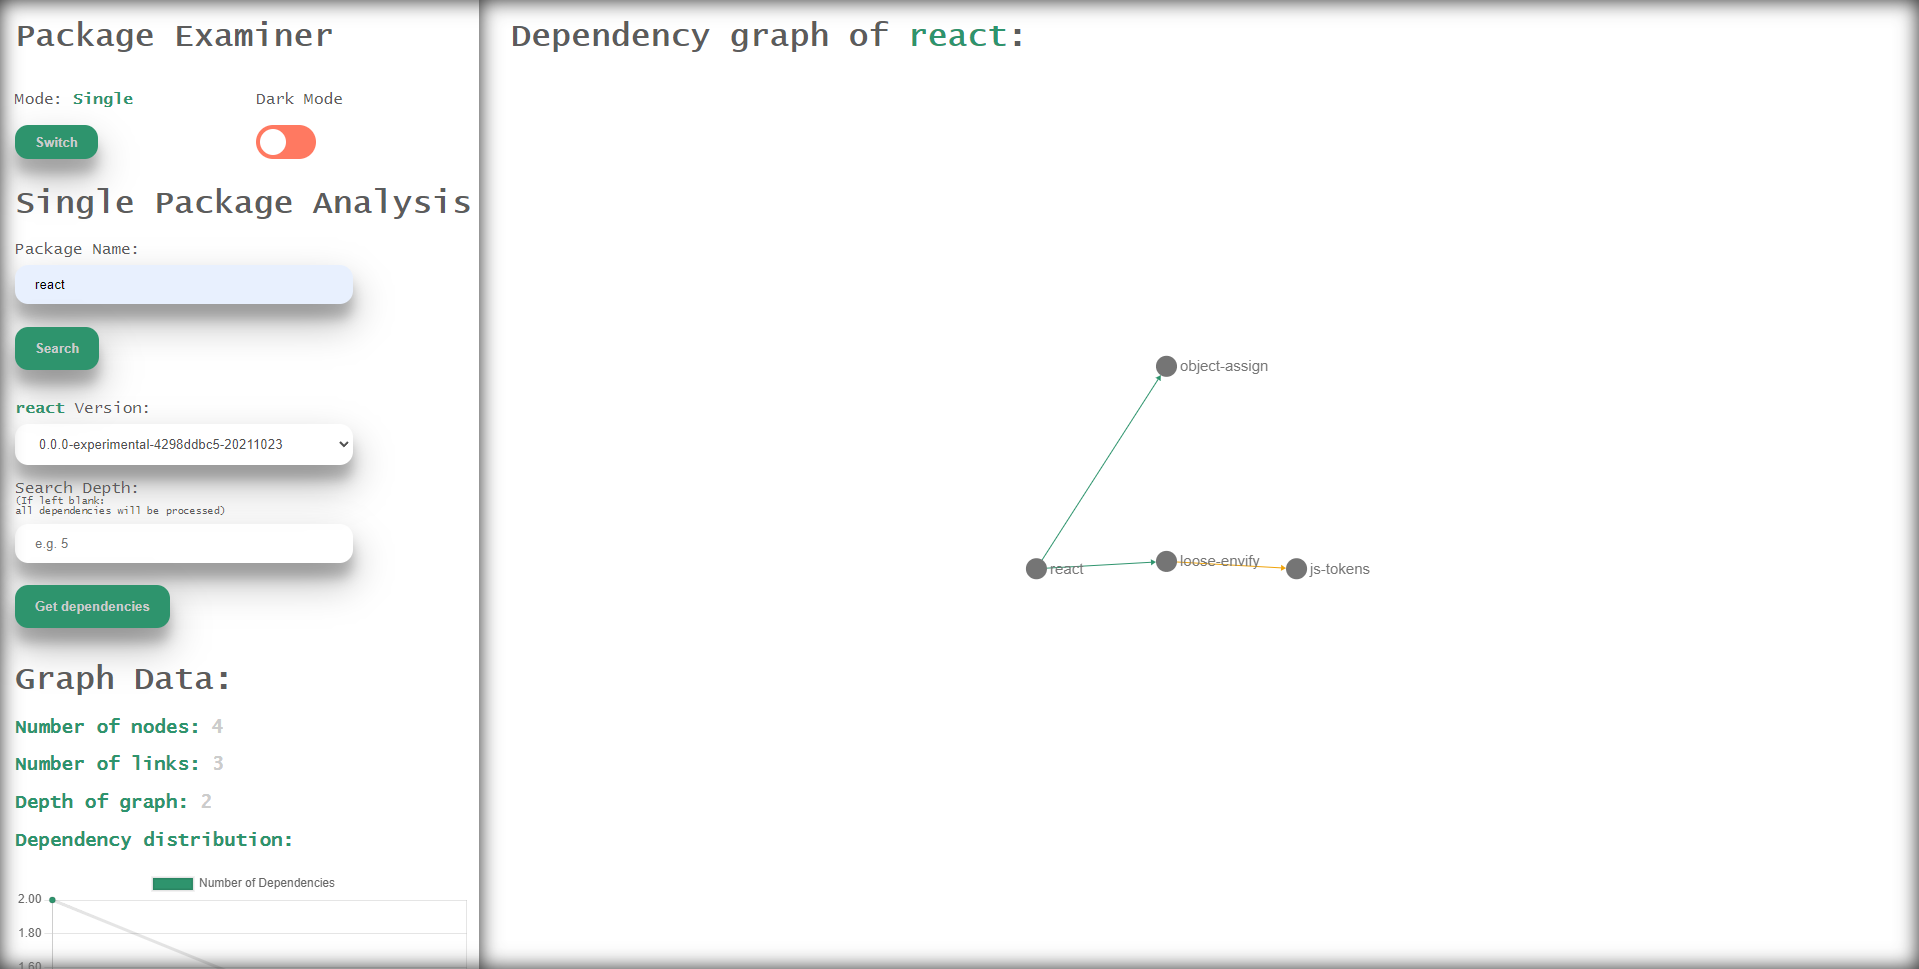
\includegraphics[scale=0.2]{images/examiner.png}
	\caption{Egy Csomagos Mód}
	\label{fig:examiner}
\end{figure}

\begin{itemize}
	\item Első lépésként meg kell adni a csomag nevét és keresni a (Search) gombbal.
	\item Helyes csomagnév esetén feltöltődik a verziók listája, innen tetszőlegesen kell választani egyet.
	\item Opcionálisan megadható, hogy keresés mennyire legyen mély
	\item Végül a (Get dependencies) gomb megnyomásával lehet elindítani a folyamatot.
	\item Az elkészült ábra görgővel és egérgomb lenyomva tartásával interaktívan mozgatható, nagyítható. A Sidebar pedig lefelé görgethető a gráfelemzés információinak megtekintéséhez.
\end{itemize}

\pagebreak

\textbf{A két mód közötti váltást a (Switch) gomb segítségével lehet megtenni.}

\begin{figure}[!h]
	\centering
	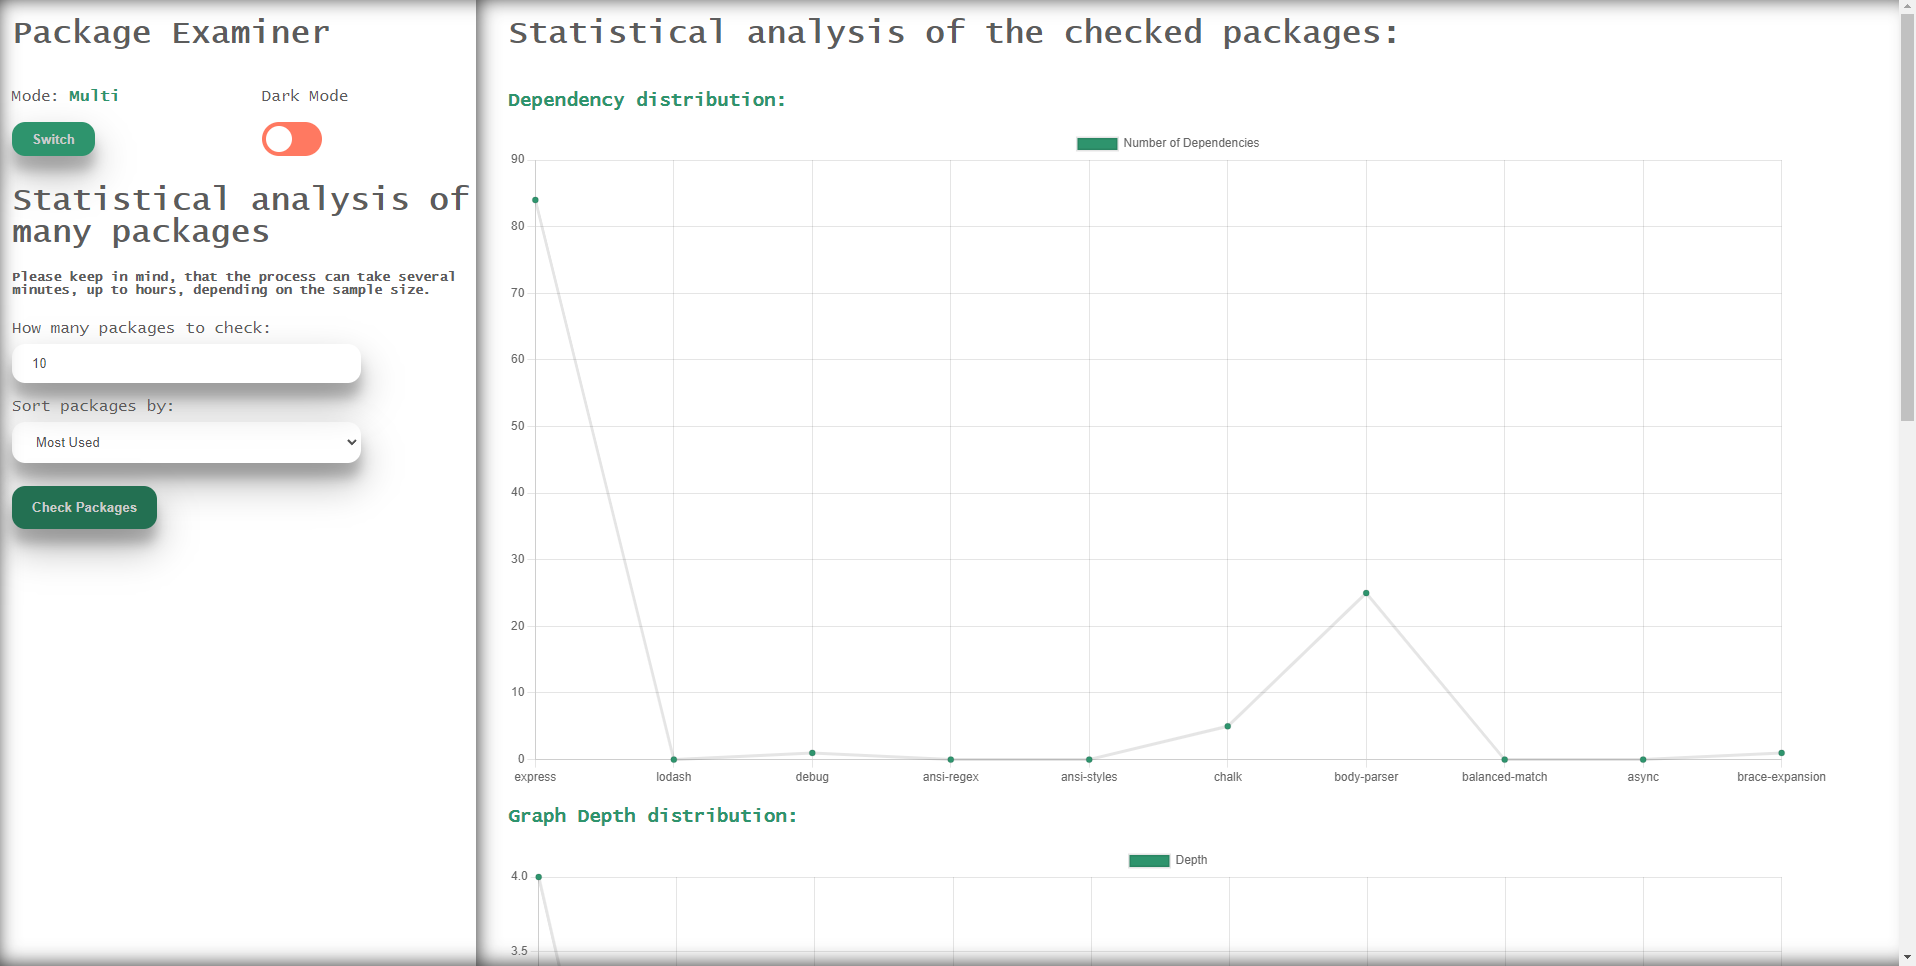
\includegraphics[scale=0.2]{images/statistics.png}
	\caption{Több Csomagos Mód}
	\label{fig:examiner}
\end{figure}

\begin{itemize}
	\item Először a vizsgált csomagok mennyiségét szükséges megadni.
	\item A lefelé gördülő listából pedig a sorrendbe állítási elvet kell kiválasztani, alapértelmezett a leggyakrabban használt csomagok elve.
	\item A folyamatot a (Check Packages) gombra kattintással lehet elindítani.
\end{itemize}

\Section{Eredmények}

A korábban tárgyalt mérete és csomagmennyisége miatt az npm Registry egészét túl hosszas és költségigényes lenne elemezni, így az első ezer leggyakrabban használt csomagról, mint "reprezentatívan leszűkített Registryről" készült statisztikai elemzés. A vizsgálat előtt a program a \textbf{csomagokat a függőségek száma szerint csökkenő sorrendbe állította}, majd elvégezte a szükséges számításokat és az eredményeket a következő hisztogramokon ábrázolta:

\begin{figure}[!h]
	\centering
	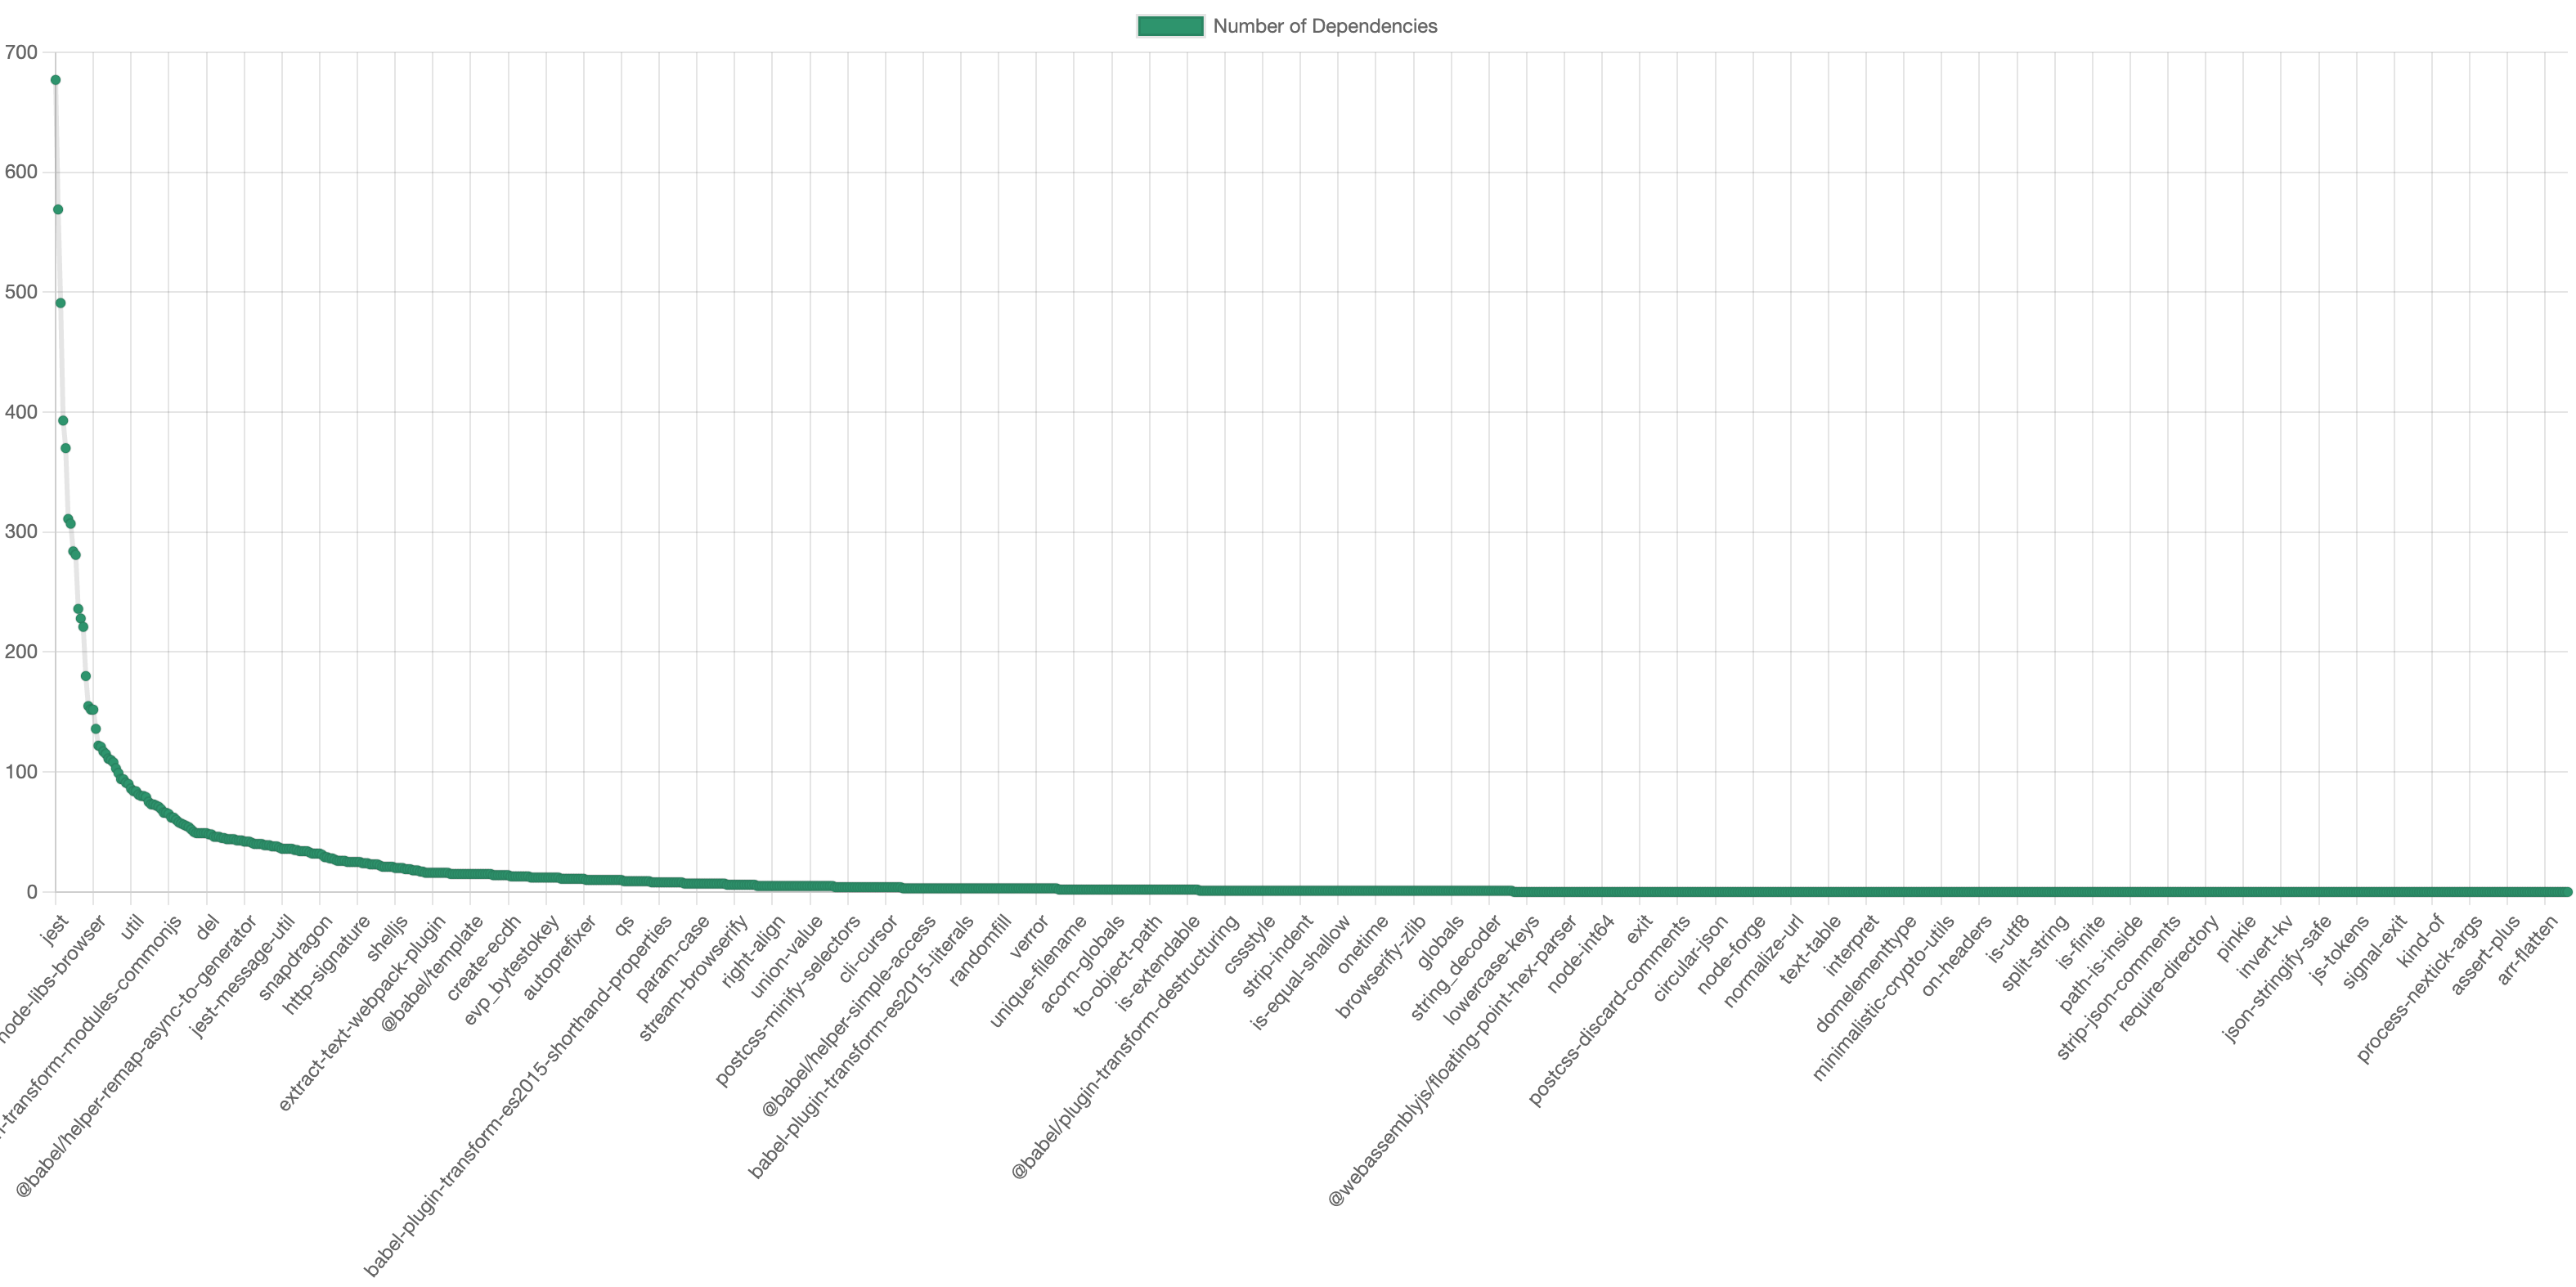
\includegraphics[scale=0.12]{images/depdist.png}
	\caption{Függőségek számának eloszlása}
	\label{fig:depdist}
\end{figure}  

\begin{figure}[!h]
	\centering
	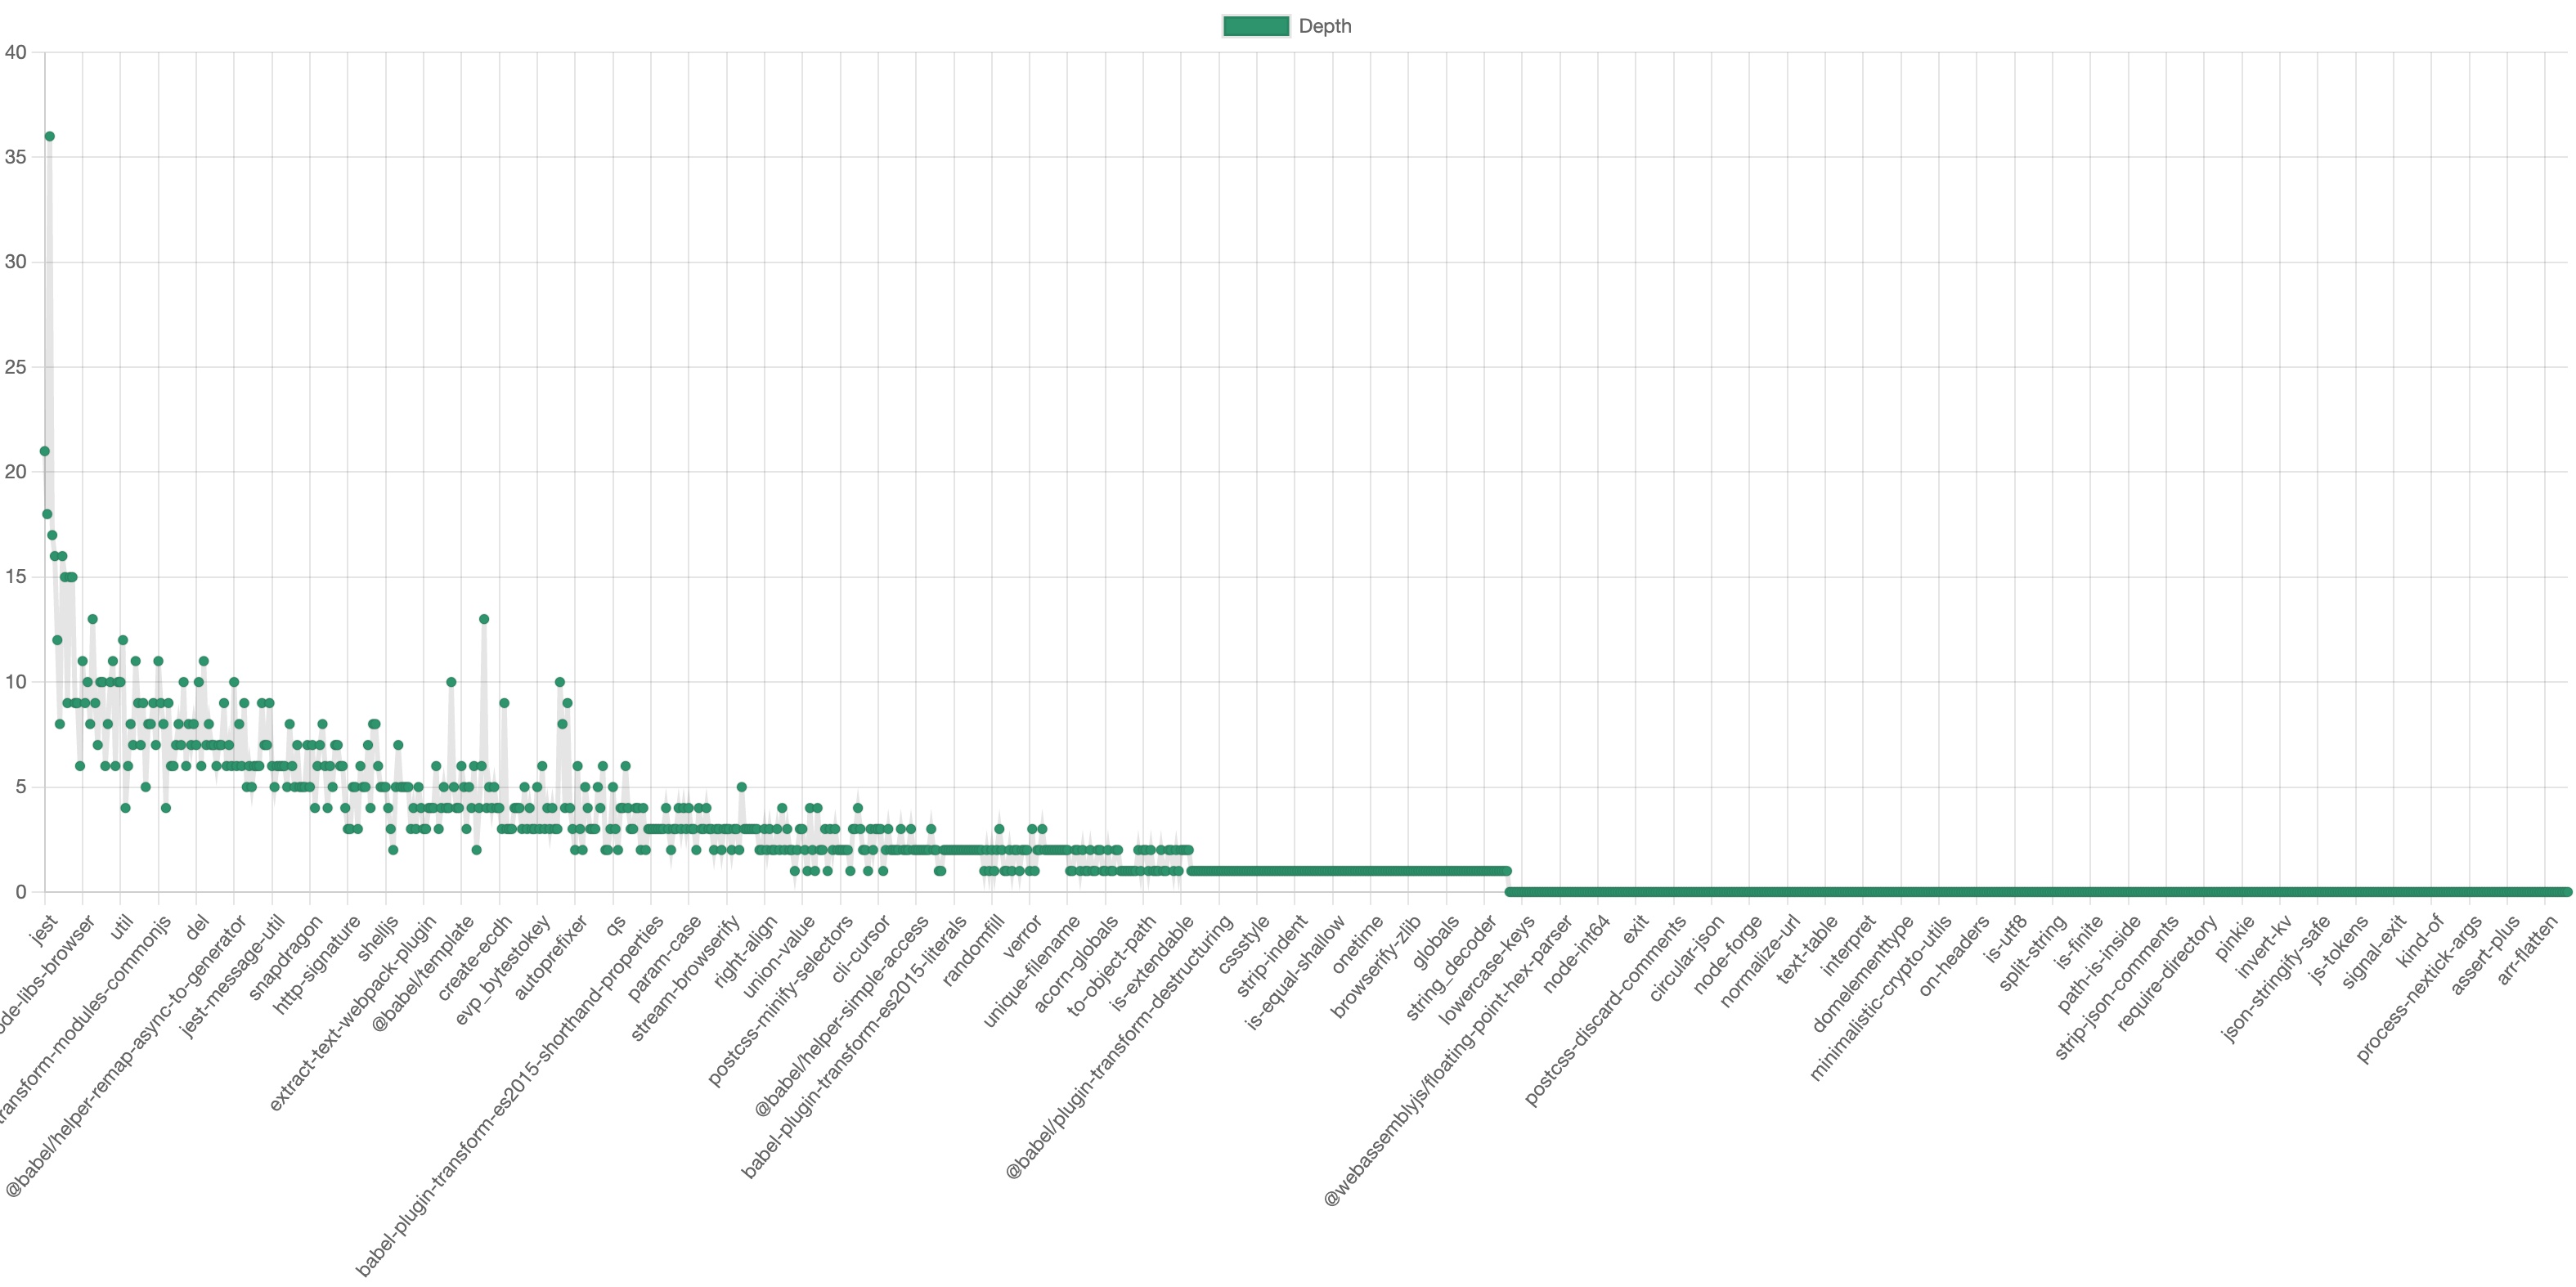
\includegraphics[scale=0.12]{images/graphdepth.png}
	\caption{Csomagonkénti gráfmélység}
	\label{fig:graphdepth}
\end{figure}

\begin{figure}[!h]
	\centering
	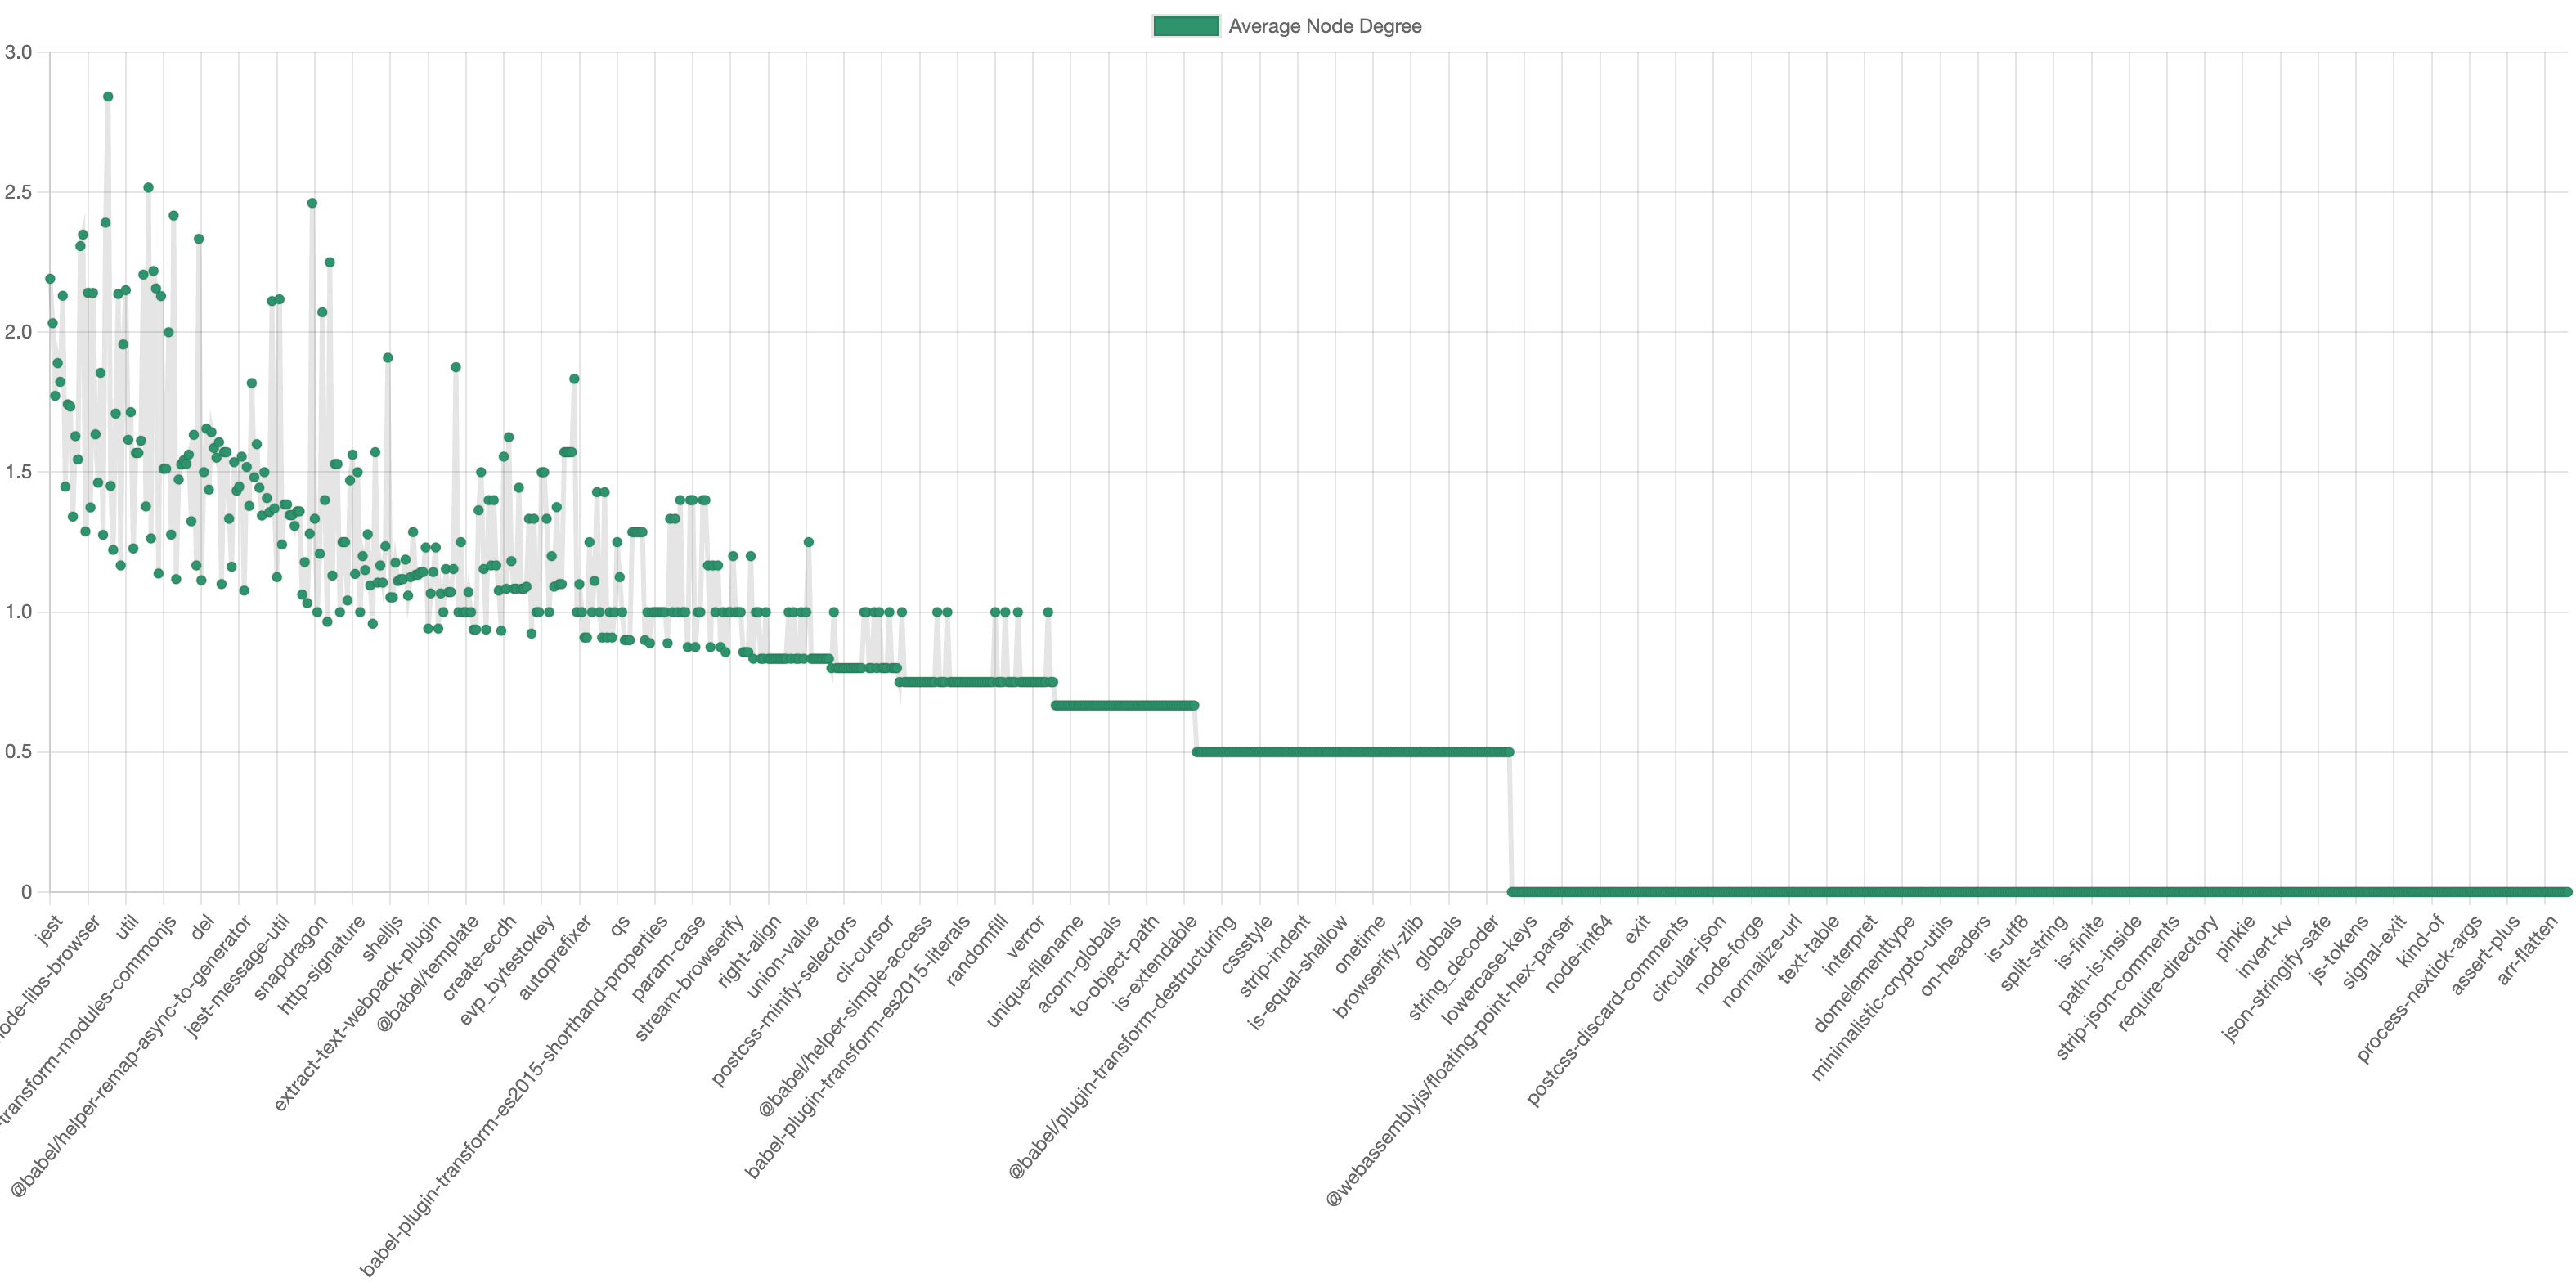
\includegraphics[scale=0.12]{images/avgdegree.png}
	\caption{Csomagonkénti átlagos fokszám}
	\label{fig:avgdegree}
\end{figure}

\begin{figure}[!h]
	\centering
	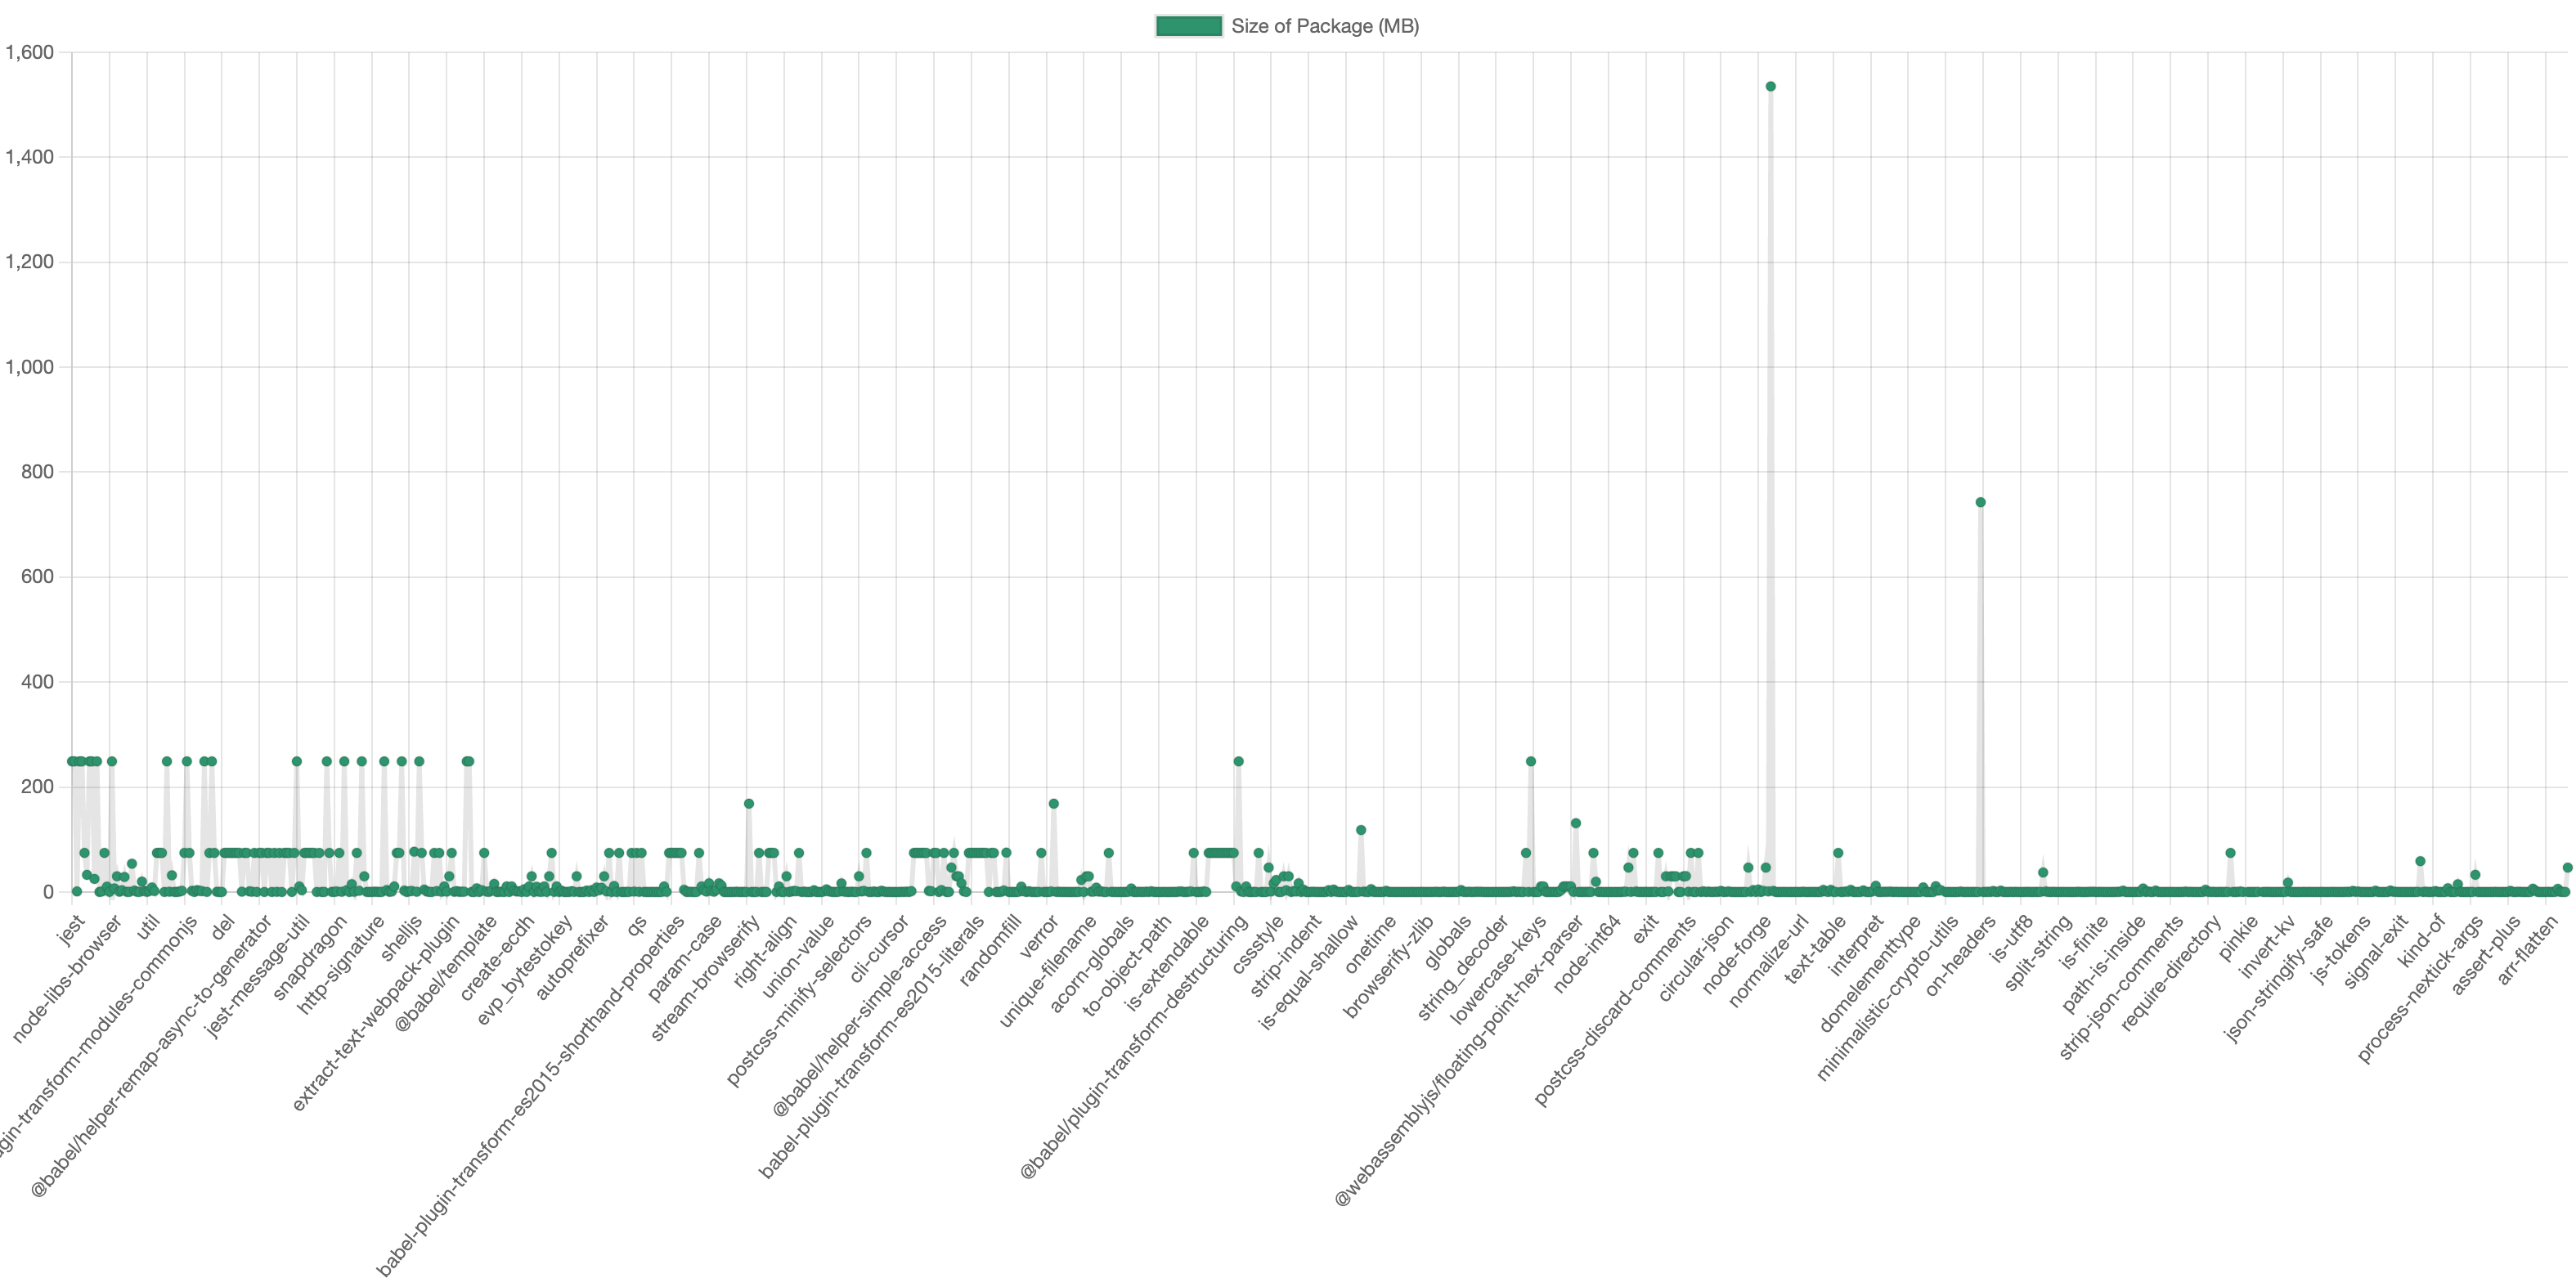
\includegraphics[scale=0.12]{images/pkgsize.png}
	\caption{Csomagméret(MB-ban megadott) eloszlás}
	\label{fig:pkgsize}
\end{figure}

\begin{figure}[!h]
	\centering
	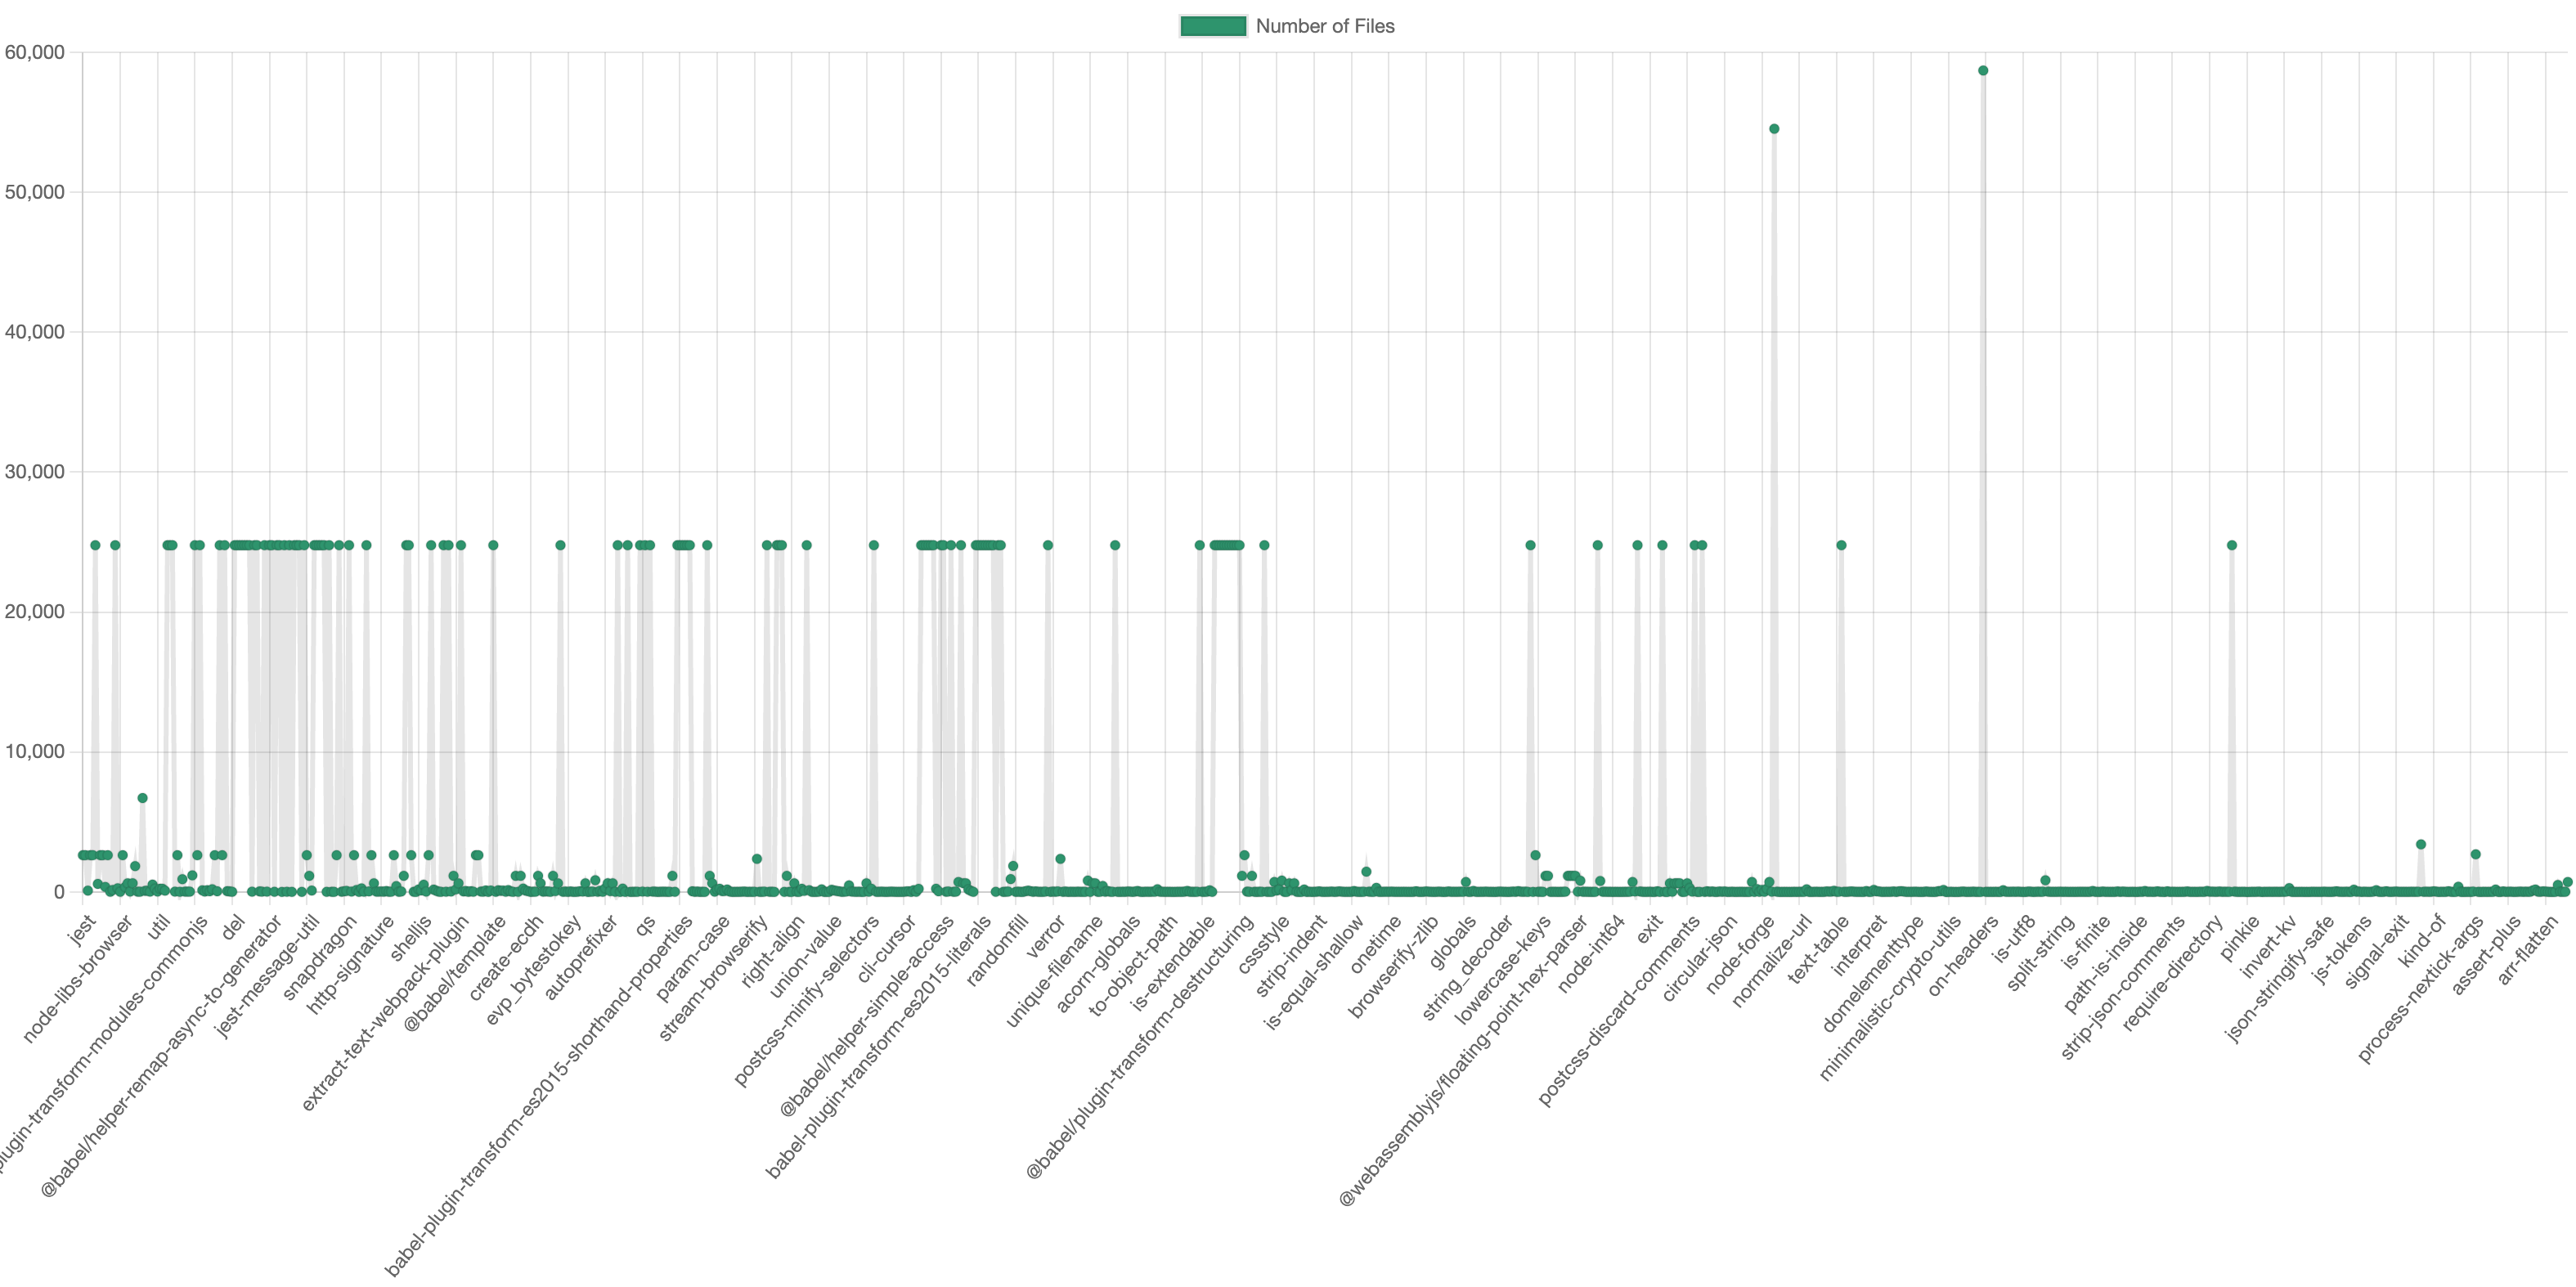
\includegraphics[scale=0.12]{images/numoffiles.png}
	\caption{Csomagonkénti fájlok száma}
	\label{fig:numoffiles}
\end{figure}

\begin{figure}[!h]
	\centering
	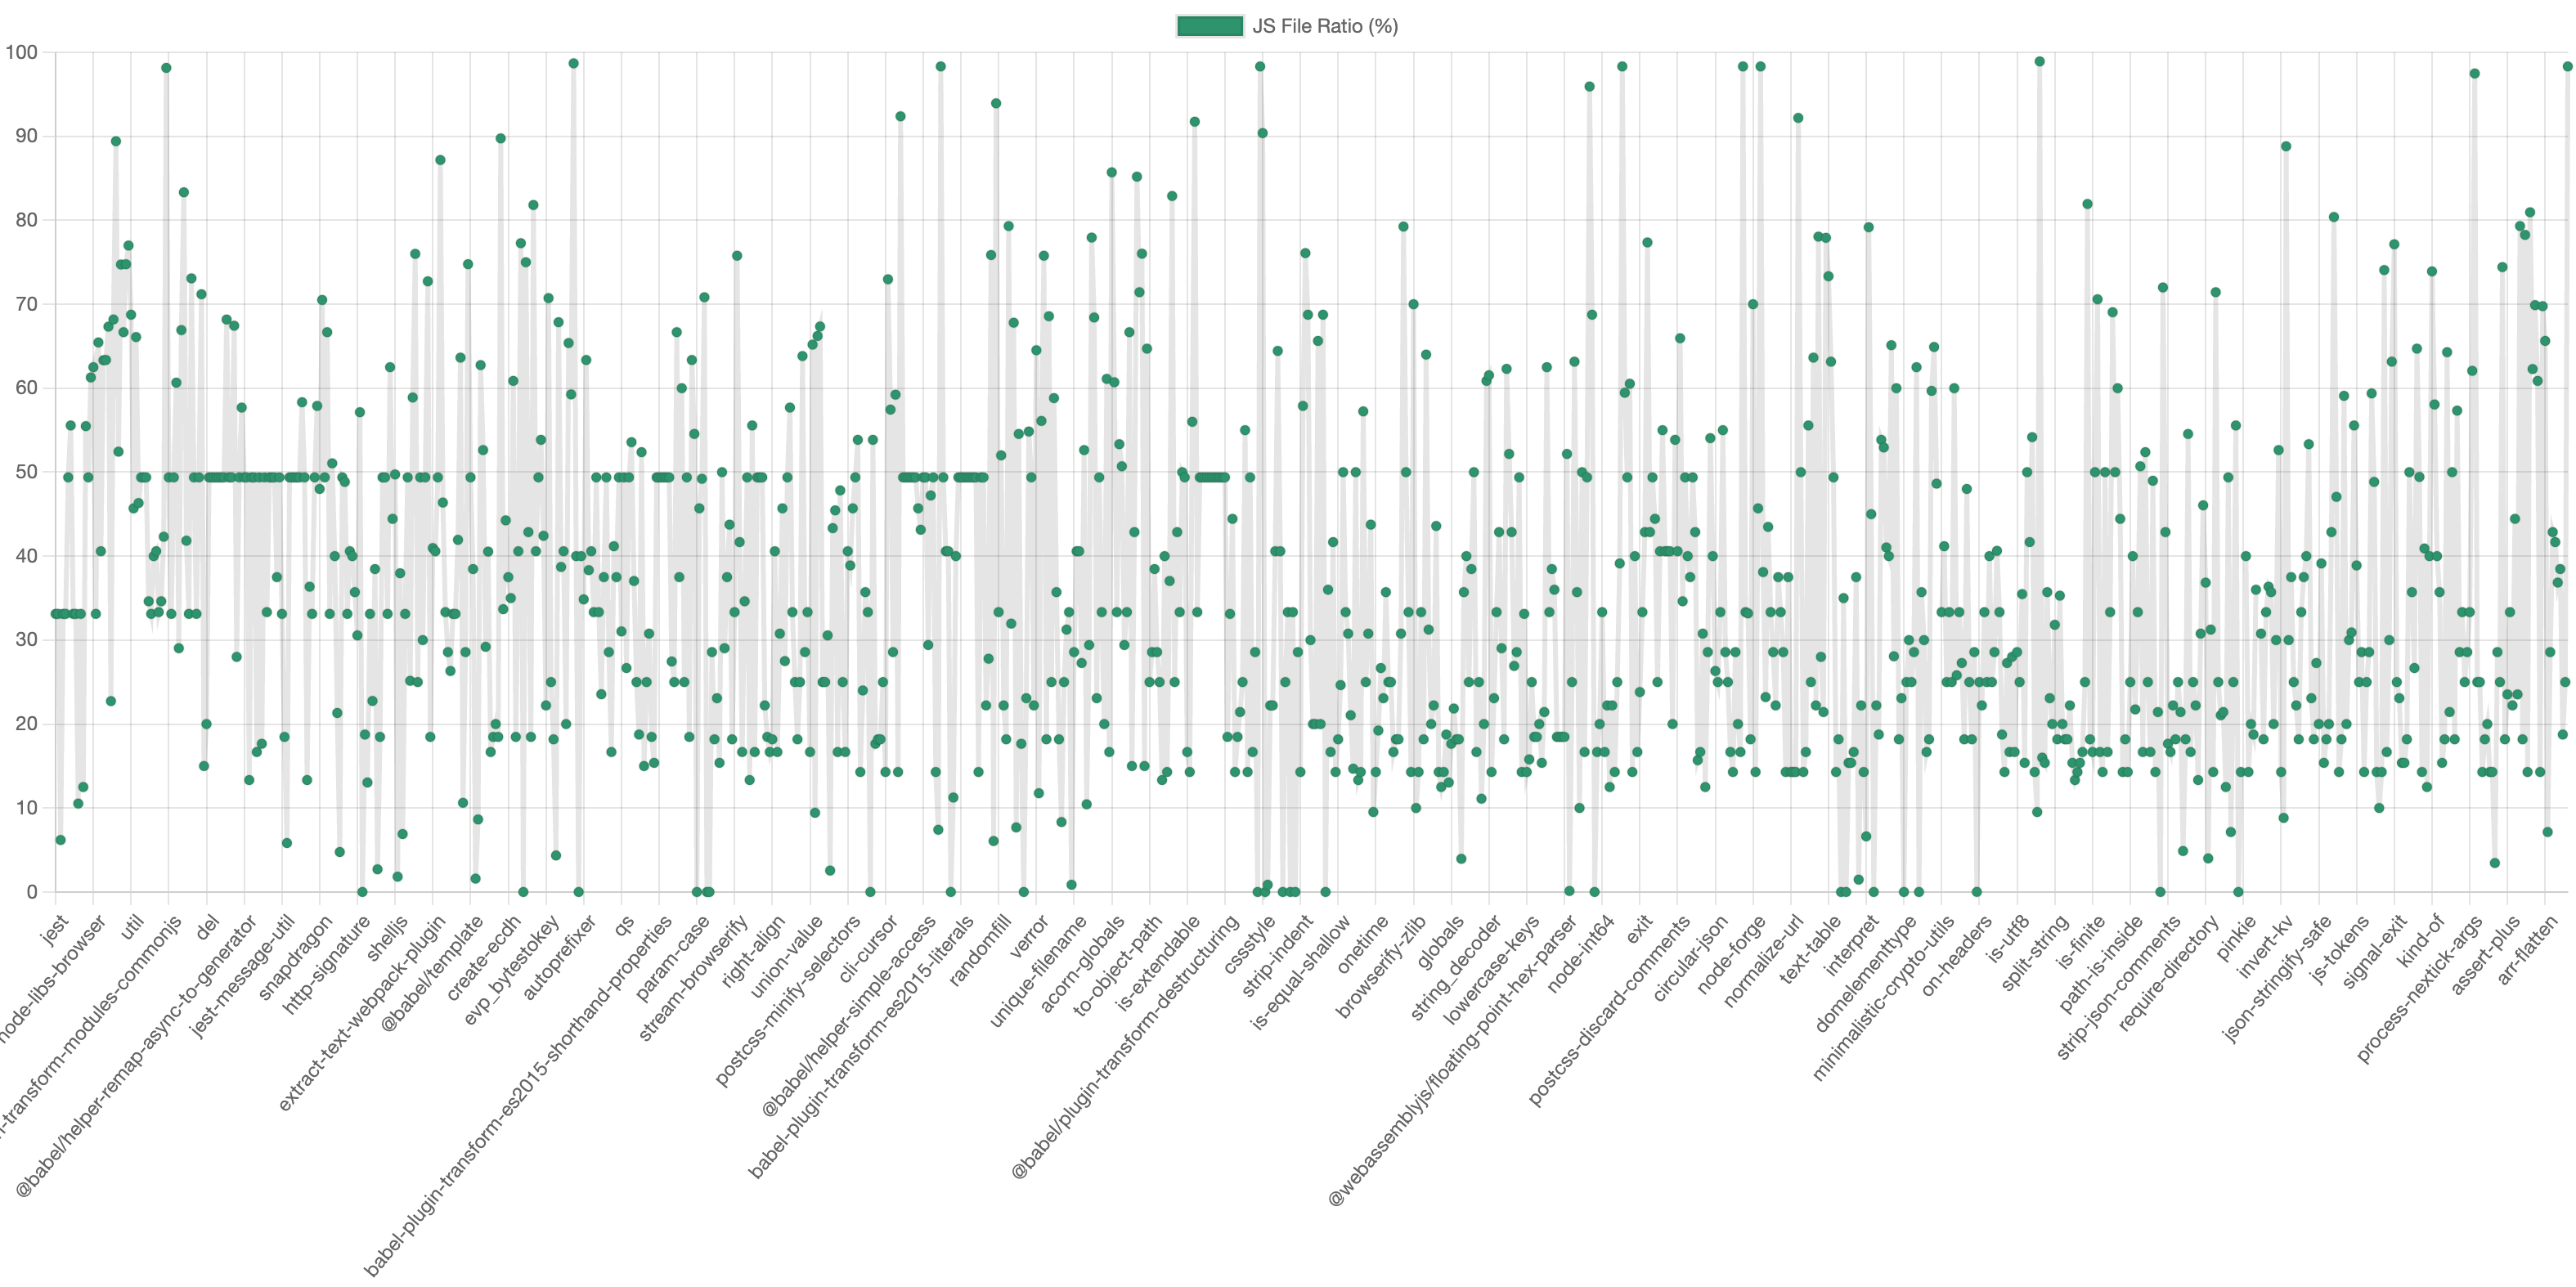
\includegraphics[scale=0.12]{images/jsratio.png}
	\caption{Csomagonkénti JavaScript fájlok aránya (\%)}
	\label{fig:jsratio}
\end{figure}

\begin{figure}[!h]
	\centering
	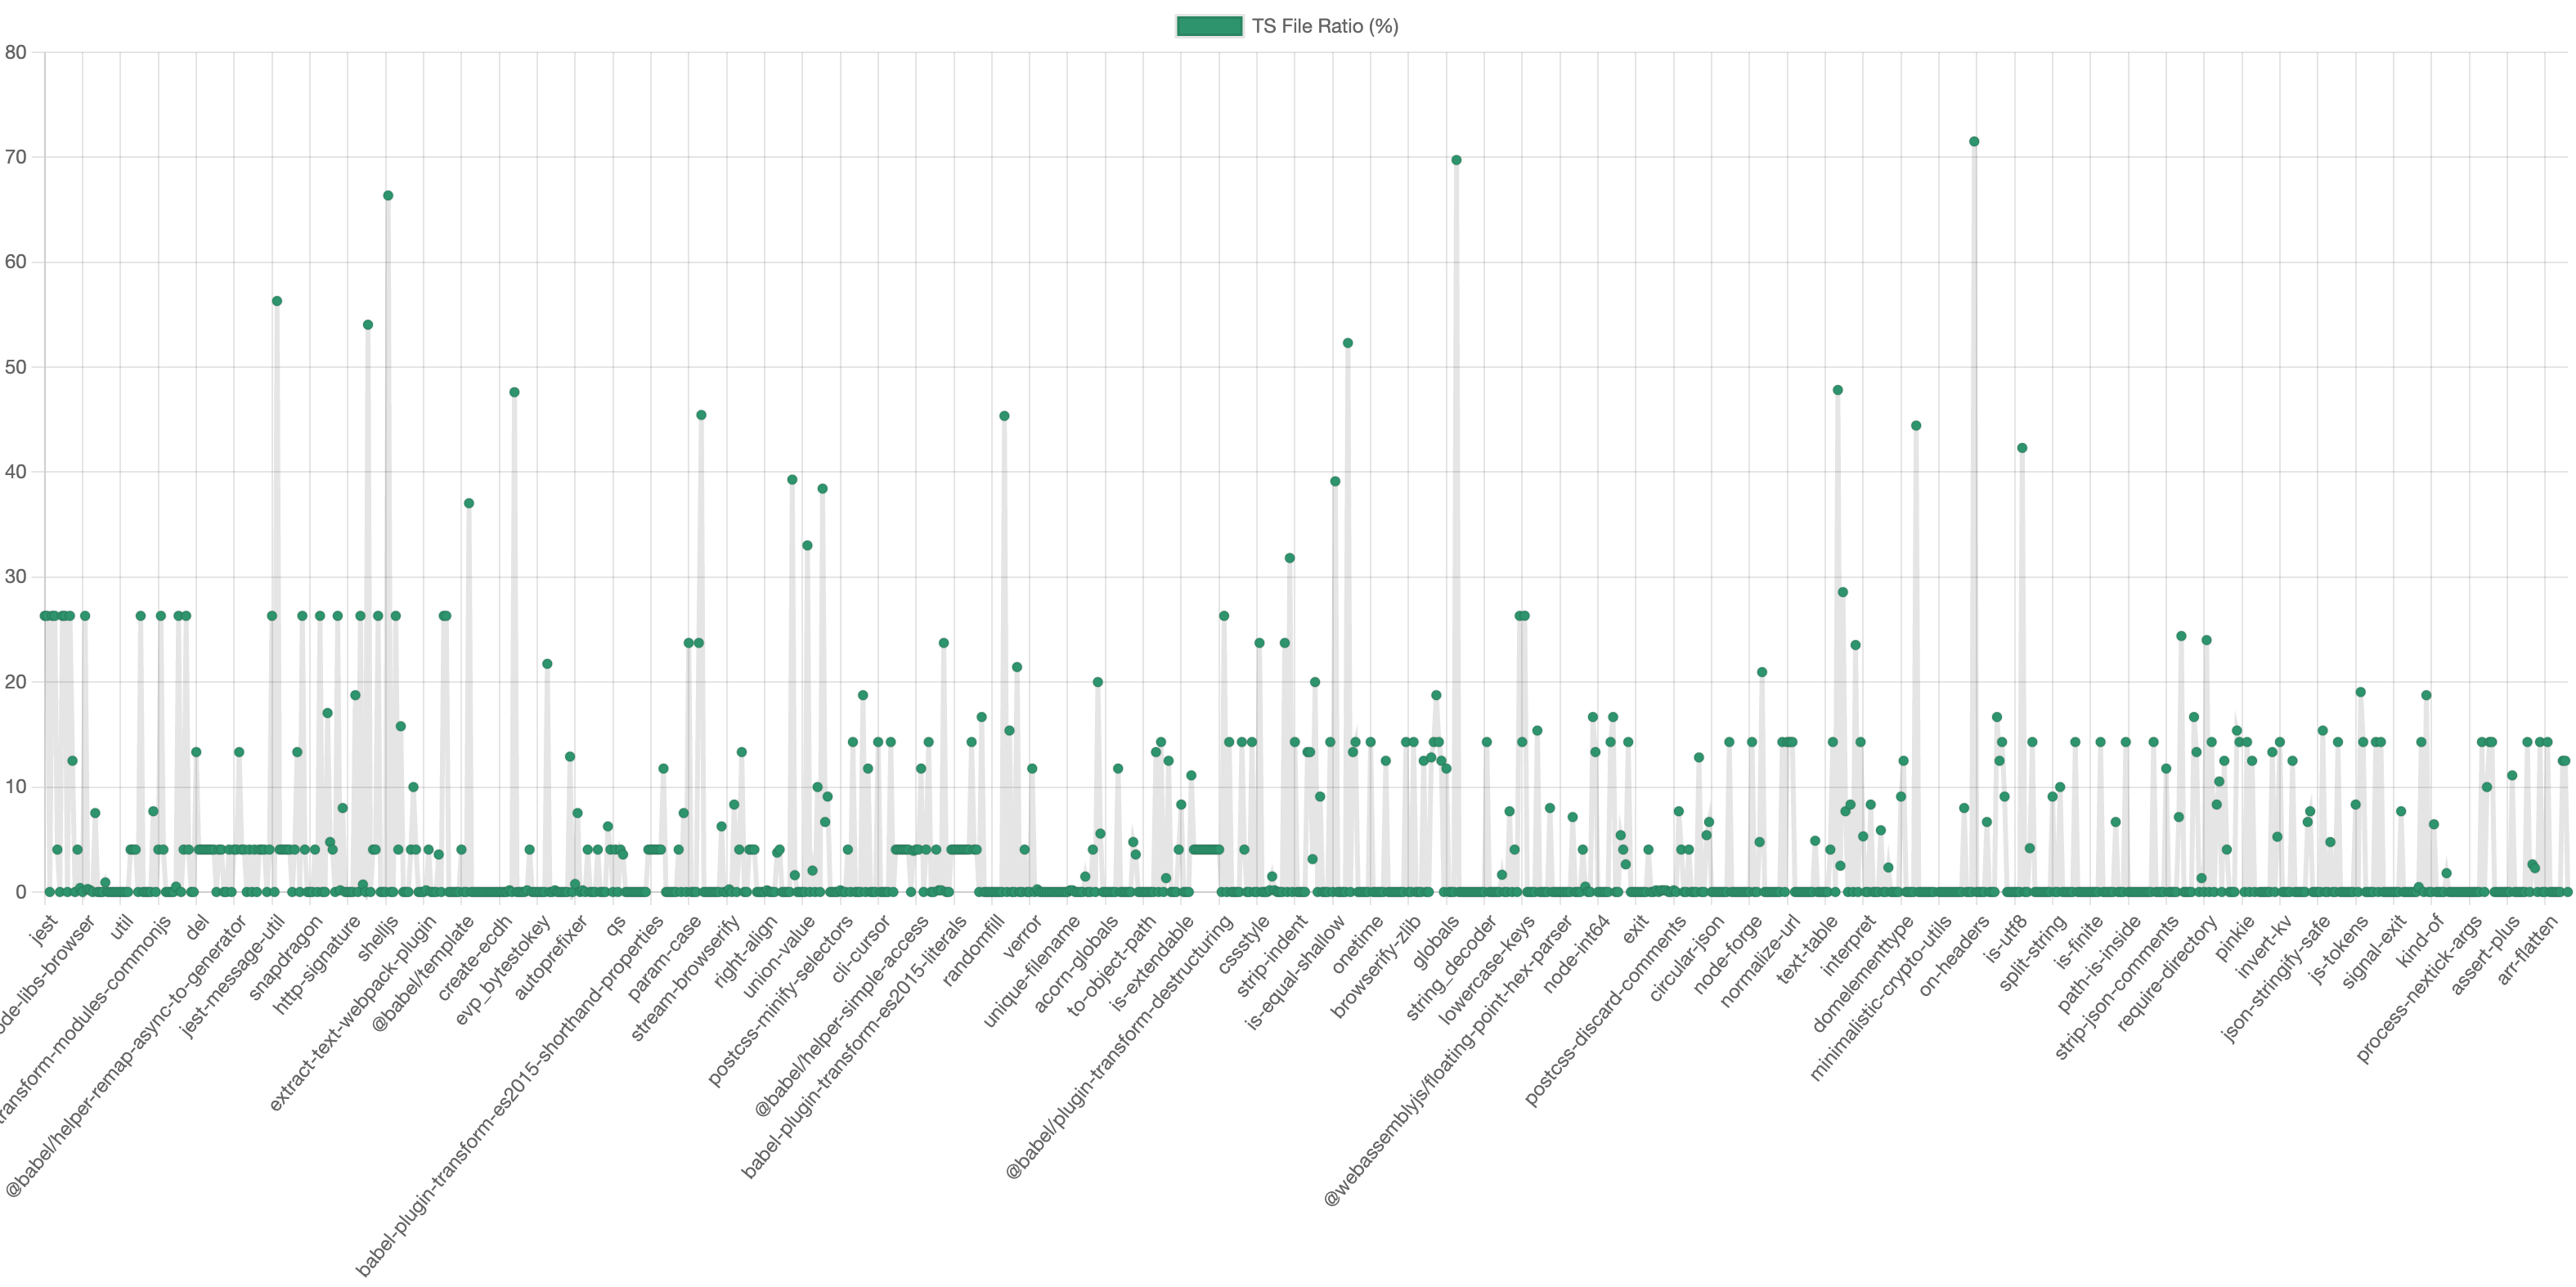
\includegraphics[scale=0.12]{images/tsratio.png}
	\caption{Csomagonkénti TypeScript fájlok aránya (\%)}
	\label{fig:tsratio}
\end{figure}

\pagebreak

\subsubsection{Eredmények Elemzése}

A program a számított hisztogramokat maga is elemezte, minden ábra esetében kiszámolta a prezentált adatok átlagát és szórását, melyet a Sidebar-ra írt ki az alábbi módon (Average = Átlag, Standard Deviation = Szórás):

\begin{figure}[!h]
	\centering
	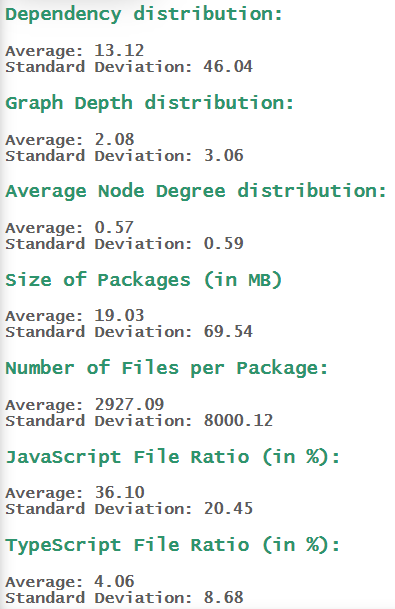
\includegraphics[scale=0.35]{images/hg_data.png}
	\caption{Hisztogramok Elemzése}
	\label{fig:hg_data}
\end{figure}

A vizsgálat során minden csomag esetében a legutóbbi stabil verziót vette alapul a program. 

Az számítások és ábrázolás előtt a program \textbf{a csomagokat a függőségek száma szerinti csökkenő sorrendbe rendezte}, hogy egyértelműbbek legyenek az esetleges összefüggések.

\begin{itemize}
	\item Természetesen a gráf mélysége és a csomagok átlagos fokszáma, bár nem szigorúan, de követte a függőségek számának változását.
	\item A csomagméret esetében már ez a tendencia nem jelenik meg, bár alapvetően a nagyobb mennyiségű függőség esetében gyakoribb a nagy csomagméret.
	\item A csomagokban található fájlok mennyisége változó, de részben indikálja a csomag méretét.
	\item A JavaScript és TypeScript fájlok aránya az összes fájlhoz képest erősen inkonzisztens. Alapvetően elmondható, hogy a JavaScript alapú csomagok jóval gyakoribbak, mint a TypeScript alapúak.
\end{itemize}

\subsubsection{Érdekességek, kiugrások az ábrákon:}

\begin{itemize}
	\item \textbf{Függőségek száma:} A legtöbb (400 feletti) függőséggel a \textbf{jest} (677), \textbf{jest-config} (569) és \textbf{gulp} (491) rendelkezik.
	\item \textbf{Gráf mélysége:} A \textbf{jest} 21 mélységű függőségi gráffal rendelkezik, amelyet indokol a függőségeinek száma, azonban a \textbf{gulp} érdekesebb, itt a kirívó 36-os mélység annak köszönhető, hogy található függőségi gráfjában nem várt kör, amely miatt az algoritmus tovább próbálta rendezni, sikertelenül a pontokat, míg végül feladta.
	\item \textbf{Átlagos fokszám}:  A \textbf{crypto-browserify} a maga 2.842-es átlagával volt a legmagasabb, de kirívónak nem nevezhető.
	\item \textbf{Csomagméret:} Két feltűnően nagy méretű csomag a \textbf{typescript} (1.541,57 MB) és a \textbf{@types/node} (746,19 MB) amik maguk a TypeScript csomag és a Type-Script által használt Node.JS típusdefiníciókat tartalmazó csomag.
	\item \textbf{Fájlok száma:} Természetesen a két legnagyobb csomag kirívó itt is: \textbf{typescript:} 54.554 fájl, \textbf{@types/node:} 58.643 fájl.
	\item \textbf{TypeScript arány:} A JavaScript fájlok aránya változó, nincs kifejezetten kirívó eset, viszont a TypeScript esetében a \textbf{@types/node} típusdefiníciók 71,45\%-a TS fájl, illetve az ajv-keyword 79,74\%-a.
	\item \textbf{jest és babel: }A jest és babel scope-pal rendelkező csomagok és alcsomagok mind ugyanarra a GitHub linkre mutatnak a package.json fájlban, mivel ugyanazon repositoryban található minden alcsomag, így a fájlszintű elemzések esetében (csomagméret, fájlok száma, TS és JS arányok) ugyanazokat az értékeket hozzák. Ez magyarázza ezeknél az ábráknál a több azonosan magas pontot.
	
\end{itemize}


\Section{Önelemzés}

A szoftver Node.JS csomagként is működik, a publikus npm registry-ben kiadásra került. Ennek köszönhetően a program tudja a saját függőségeit elemezni, amelyre az alábbi eredményt adta:

\begin{itemize}
	\item A függőségként megjelölt és használt 3 csomag közül a szemantikus verziózásért felelős semver két további függőségi szintet eredményezett, amely nem lett volna egyértelmű pusztán a package.json tartalma alapján.
	\item Az elemzés során nem talált kulcsszavakban rejlő redundáns funkcionalitásra jeleket.
\end{itemize}

\begin{figure}[!h]
	\centering
	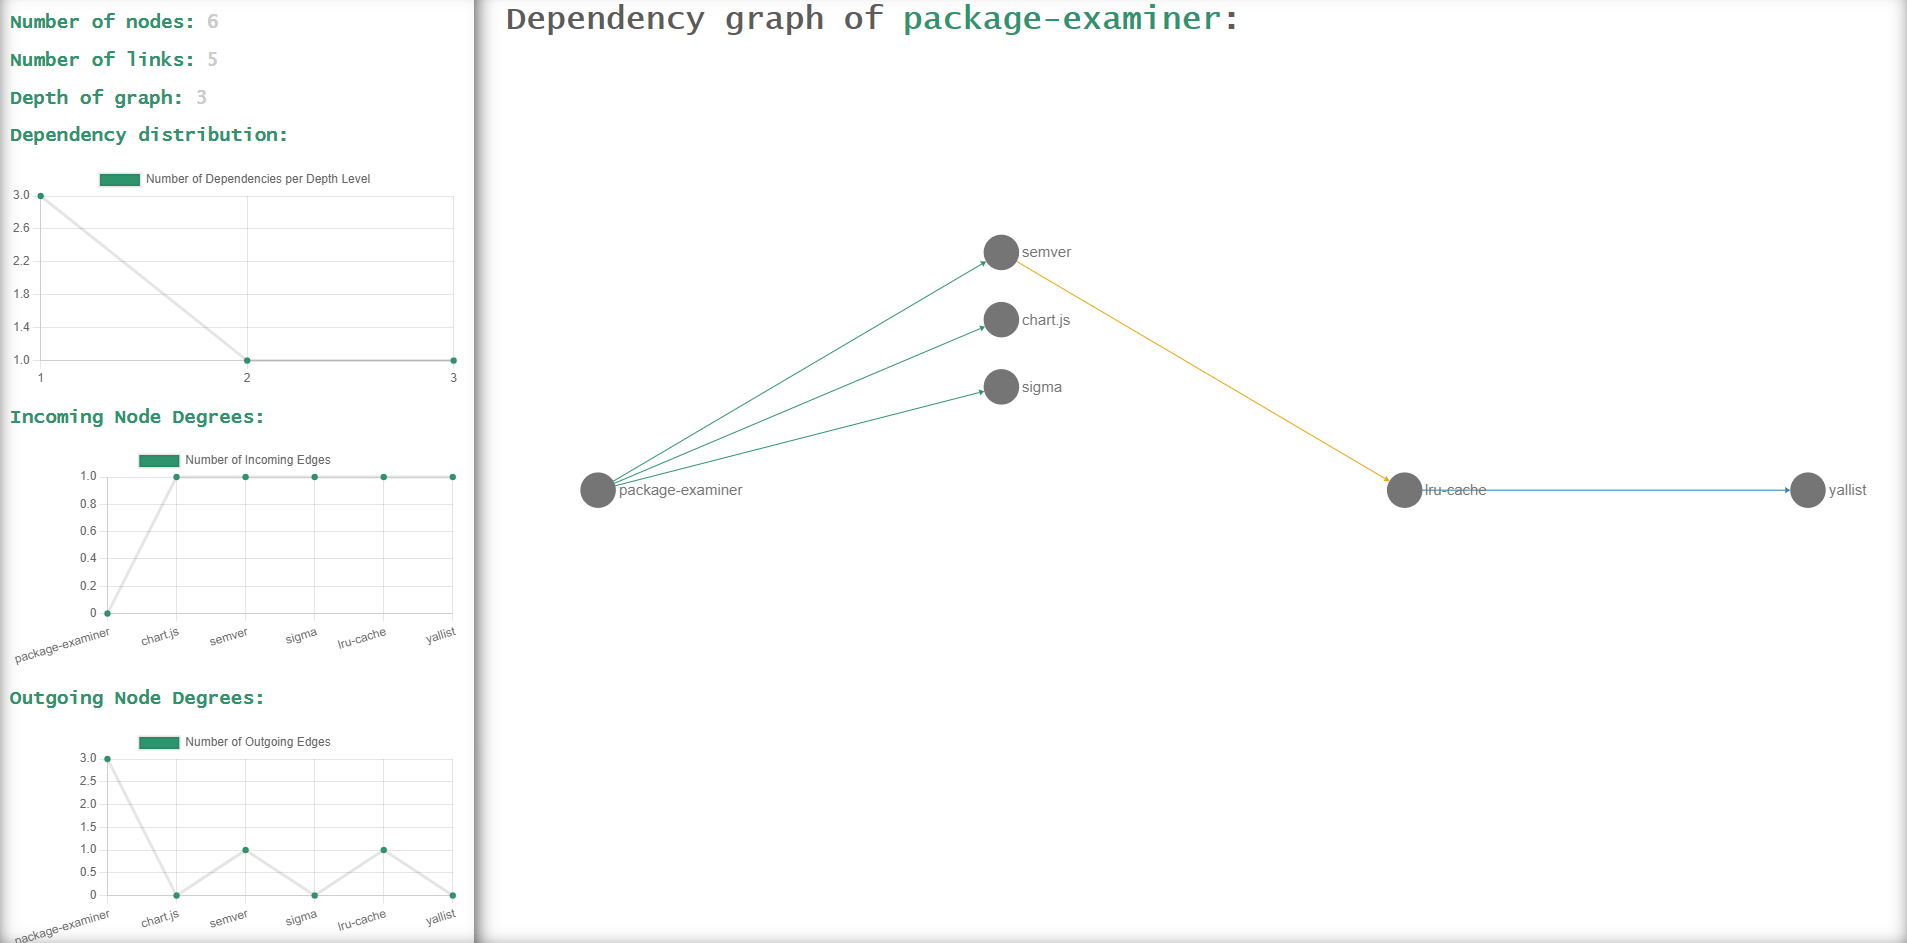
\includegraphics[scale=0.25]{images/package-examiner.png}
	\caption{A Package Examiner függőségeinek elemzése}
	\label{fig:package-examiner}
\end{figure}